\chapter{Indefinite quadratic forms}\label{chap3}

\section{Discontinuous groups}\label{chap3:sec1}\pageoriginale

In the previous chapter we had met with the situation in which a group
of transformations acts on a topological space and we constructed, by
a certain method, a subset of this space which has some distinguished
properties relative to the group. We shall now study the following
general situation.

Let $\Gamma$ be an abstract group and $T$ a Hausdorff topological
space on which $\Gamma$ has a representation
\begin{equation*}
t\to t\gamma,\quad t\in T,\quad \gamma\in\Gamma\tag{1}\label{c3:eq1}
\end{equation*}
carrying $T$ into itself. We say that this representation of $\Gamma$
is {\em discontinuous} if for every point $t\in T$, the set of points
$\{t\gamma\}$ for $\gamma\in\Gamma$ has no limit point in $T$. The
problem now is to determine, for a given $\Gamma$, all the spaces $T$
on which $\Gamma$ has a discontinuous representation. For an
arbitrarily given group, this problem can be very difficult. We shall,
therefore, impose certain restrictions on $\Gamma$ and $T$. Let us
assume that there is a group $\Omega$, of transformations of $T$ onto
itself, which is {\em transitive} on $T$. This means that if $t_{1}$
and $t_{2}$ are any two elements of $T$, there exists
$\omega\in\Omega$ such that
\begin{equation*}
t_{1}=t_{2}\omega.\tag{2}\label{c3:eq2}
\end{equation*}
Let us further assume that $\Gamma$ is a subgroup of $\Omega$. Let
$t_{0}$ be a point in $T$ and consider the subgroup $\Lambda$ of
$\Omega$ consisting of $\lambda \in\Omega$ such\pageoriginale that
\begin{equation*}
t_{0}=t_{0}\lambda.\tag{3}\label{c3:eq3}
\end{equation*}
If $t$ is any point of $T$, we have because of transitivity,
$$
t=t_{0}\rho
$$
for some $\rho\in\Omega$. Because of \eqref{c3:eq3}, we get
$$
t=t_{0}\Lambda\rho.
$$
Conversely if $\rho'\in\Omega$ is  such that
$t=t_{0}\rho'$, then $t_{0}\rho'=t_{0}\rho$ or
$\rho'\in\Lambda_{\rho}$. Thus every point $t\in T$ determines a coset
$\Lambda_{\rho}$ of $\Lambda\backslash \Omega$ that is, the space of
right cosets of $\Omega$ modulo $\Lambda$. Conversely if
$\Lambda_{\rho}$ is any coset, then $t=t_{0}\rho$ is a point
determined by $\Lambda_{\rho}$. Hence the mapping
\begin{equation*}
t\to \Lambda_{\rho}\tag{4}\label{c3:eq4}
\end{equation*}
of $T$ on $\Lambda\backslash \Omega$ is $(1,1)$ both ways. In order to
make this correspondence topological, let us study the following
situation.

Let $\Omega$ be locally compact topological group and $T$ a Hausdorff
topological space on which $\Omega$ has a representation
\begin{equation*}
t\to t\omega\tag{5}\label{c3:eq5}
\end{equation*}
as a transitive group of mappings. Let us assume that this
representation is open and continuous. We recall that \eqref{c3:eq5} is
said to be {\em open} if for every open set $P$ in $\Omega$ and every
$t\in T$ the set $\{t\omega\}$, $\omega\in P$ is an open set in
$T$. Then it follows that the subgroup $\Lambda$ of $\Omega$ leaving
$t_{0}\in T$ fixed is not only a closed subgroup but that the mapping
\eqref{c3:eq4} of $T$ on $\Lambda\backslash \Omega$ is a homeomorphism.

Let\pageoriginale $\Gamma$ be a subgroup of $\Omega$ which has on $T$
a discontinuous representation. Then $\Gamma$ has trivially a
representation in $\Lambda\backslash \Omega$. By the remarks above,
the representation
\begin{equation*}
\Lambda\omega\to \Lambda\omega\rho,\quad \rho\in\Gamma\tag{6}\label{c3:eq6}
\end{equation*}
is discontinuous in $\Lambda\backslash \Omega$.

On the other hand, let $\Lambda$ be {\em any} closed subgroup of
$\Omega$. Then the representation
$$
\omega'\to \Lambda\omega\omega'
$$
of $\Omega$ on $\Lambda\backslash\Omega$ is open and continuous. It is
clearly transitive. In order, therefore, to find all spaces on which
$\Gamma$ has a discontinuous representation, it is enough to consider
the spaces of right cosets of $\Omega$ with regard to closed subgroups
$\Lambda$ of $\Omega$.

Suppose $\Lambda$ is a closed subgroup of $\Omega$ and $\Gamma$ has a
discontinuous representation on $\Lambda\backslash\Omega$. Let $K$ be
a closed subgroup of $\Omega$ contained in $\Lambda$. Then $\Gamma$
has a discontinuous representation on $K\backslash\Omega$. For, if
$K\omega$ is a coset such that the set of cosets $\{K\omega\rho\}$,
$\rho\in\Gamma$ has a limit point in $K\backslash\Omega$, then the set
$\{\Lambda\omega\rho\}$, $\rho\in\Gamma$ also has a limit point in
$\Lambda\backslash\Omega$ and so \eqref{c3:eq6} would not be
discontinuous. In particular, if we take for $K$ the subgroup
consisting only of the identity element $\ub{e}$, then $\Gamma$ is
discontinuous in $\Omega$ is clearly equivalent to $\Gamma$ is a {\em
  discrete} subgroup of $\Omega$.

Thus if there exists some subgroup $\Lambda$ of $\Omega$ such that
$\Gamma$ is discontinuous in $\Lambda\backslash\Omega$, then
necessarily $\Gamma$ has to be discrete. It can be proved that if
$\Omega$ has a countable basis of open sets, then $\Gamma$ is
enumerable.

Suppose\pageoriginale now that $\Omega$ is a locally compact group
with a countable basis of open sets. Let $\Gamma$ be a discrete
subgroup of $\Omega$. If $\Lambda$ is any compact, hence closed,
subgroup of $\Omega$ then it follows that the representation \eqref{c3:eq6}
of $\Gamma$ in $\Lambda\backslash\Omega$ is discontinuous. This can be
seen by assuming that for a certain $\omega$, the set
$\Lambda\omega\rho_{n}$, $\rho_{n}\in\Gamma$ has limit point and this
will lead to a contradiction because of the discreteness of $\Gamma$.

In general the fact \eqref{c3:eq6} is discontinuous in
$\Lambda\backslash\Omega$ does not entail that $\Lambda$ is
compact. Let us, therefore, consider the following situation.

Let $\Omega$ be a locally compact group possessing a countable basis
of open sets. Then there exists in $\Omega$ a right invariant Haar
measure $d\omega$ which is determined uniquely upto a positive
multiplicative factor. Let $\Gamma$ be a discrete subgroup of
$\Omega$. There exists then in $\Omega$ a subset $F$ possessing the
following properties: 1)~$\bigcup\limits_{a\in\Gamma}Fa=\Omega$,
2)~the sets $\{Fa\}$ for $a\in\Gamma$ are mutually disjoint and 3)~$F$
is measurable in terms of the Haar measure $d\omega$. $F$ is then said
to be a {\em fundamental} set relative to $\Gamma$. Note that if $F$
is a fundamental set then so if $Fa$ for any $a\in\Omega$ so that a
fundamental set is not unique. 1)~and 2)~assert that $F$ intersects
each coset of $\Gamma\backslash\Omega$ in exactly one point so that
$F$ has to be formed in $\Omega$ by choosing one element from each
coset $\Gamma\backslash\Omega$. The interesting point is that, under
the conditions on $\Omega$, this can be done in such a way that the
resulting set $F$ is measurable. Let us now assume that 
\begin{equation*}
\int\limits_{F}d\omega<\infty.\tag{7}\label{c3:eq7}
\end{equation*}\pageoriginale
It can then be shown that the value of the integral in \eqref{c3:eq7} is
independent of the choice of $F$. We now state, without proof, the
important

\setcounter{thm}{0}
\begin{thm}\label{chap3:thm1}
Let $\Omega$ be a locally compact topological group with a countable
basis of open sets. Let $\Gamma$ be a discrete subgroup of $\Omega$
and $F$ a fundamental set in $\Omega$ relative to $\Gamma$. Let $F$
have finite Haar measure in $\Omega$. If $\Lambda$ is any closed
subgroup of $\Omega$, then $\Gamma$ has a discontinuous representation
in $\Lambda\backslash\Omega$ if and only if $\Lambda$ is compact.
\end{thm}

The interest in the theorem lies in the {\em necessity} part of it.

Let us assume that $\Omega$ is, as will be in the applications, a Lie
group. Let $\Gamma$ be a discrete subgroup of $\Omega$. For any closed
subgroup $\Lambda$ of $\Omega$, the dimensions of $\Lambda$,
$\Lambda\backslash\Omega$ and $\Omega$ are connected by
$$
\dim\Lambda+\dim \Lambda\backslash\Omega=\dim\Omega. 
$$
If $F$ is a fundamental set in $\Omega$ with regard to $\Gamma$ and is
of finite measure, in terms of the invariant measure in $\Omega$, then
by Theorem \ref{chap3:thm1}, $\Gamma$ will be discontinuous in
$\Lambda\backslash\Omega$ if and only if $\Lambda$ is compact. In
order, therefore, to obtain a space $T=\Lambda\backslash\Omega$ of
smallest dimension in which $\Gamma$ has a discontinuous
representation, one has to consider a $\Lambda$ which is compact and
maximal with this property.

Let\pageoriginale us consider the following example.

Let $\Omega$ be the group of $n$-rowed real matrices $A\cdot\Omega$ is
a Lie group. Let us determine first all compact subgroups of
$\Omega$. Let $K$ be a compact subgroup of $\Omega$. If $C\in K$, then
$|C|=\pm 1$. For, the mapping $C\to|C|$ of $K$ into the multiplicative
group of real numbers is clearly topological and since $K$ is compact,
the set of images $|C|$ is a compact and so bounded subgroup of the
multiplicative group of real numbers. Thus $|C|=\pm 1$. In order to
study $K$ therefore, it is enough to study the group $\Omega_{0}$ of
real matrices $A$ with $|A|=\pm 1$. Let $\{dA\}$ denote the volume
measure in $\Omega_{0}$ so that
$$
\{dAB\}=\{dA\}
$$
for $B\in\Omega_{0}$. Let $\mathscr{M}$ be an open bounded subset of
$\Omega_{0}$. Consider the set
$$
\mathscr{G}=\bigcup_{C\in K}\mathscr{M}C.
$$
Since the sets $\mathscr{M}C$ are open, $\mathscr{G}$ is open. Since
$K$ is compact, it follows that $\mathscr{G}$ is bounded. Consider the
integral
$$
P=\int\limits_{\mathscr{G}}A'A\{dA\}.
$$
Since $A'A>0$, it follows that $P$ is positive. Also if $C$ is in $K$,
\begin{align*}
P[C] &= \int\limits_{\mathscr{G}}C'A'AC\{dA\}\\
&=\int\limits_{\mathscr{G}}A'A\{dAC^{-1}\}=P 
\end{align*}
This\pageoriginale proves that there exists a $P>0$ such that $P[C]=P$
for $C\in K$. Since $P>0$, there exists $B\in\Omega$ such that
$P=B'B$. Hence if $Q=BCB^{-1}$ then $Q'Q=E$ or $Q$ is
orthogonal. Hence $BKB^{-1}$ is a subgroup of the orthogonal group. We
have hence proved

\begin{thm}\label{chap3:thm2}
All maximal compact subgroups of $\Omega$ are conjugates of the real
orthogonal group.
\end{thm}

Let $\mathscr{P}_{0}$ denote the space of all positive real $n$-rowed
matrices of determinant 1. $\Omega_{0}$ has in $\mathscr{P}_{0}$ a
representation $P\to 
P[A]$, $P\in\mathscr{P}_{0}$, $A\in\Omega_{0}$ and this representation
is both open and continuous. Also $\Omega_{0}$ is transitive on
$\mathscr{P}_{0}$. The set of elements $A\in\Omega_{0}$ which fix the
matrix $E_{n}$ is precisely the orthogonal group $\Lambda$. By our
considerations above, $\Lambda\backslash\Omega_{0}$ is homeomorphic to
$\mathscr{P}_{0}$. So every discrete subgroup $\Gamma$ of $\Omega_{0}$
has discontinuous representation in $\mathscr{P}_{0}$. We shall
consider the subgroup $\Gamma$ consisting of unimodular matrices. That
this is discrete is clear. In the previous chapter we constructed for
$\Gamma$ in $\Lambda\backslash\Omega$ a fundamental domain
$\mathscr{R}$. We shall now construct a fundamental set for $\Gamma$
in $\Omega_{0}$.

In $\Omega_{0}$, $\Gamma$ is represented as a group of translations
$A\to AU$. Let us define the point set $F_{1}$ in $\Omega_{0}$ to
consist of matrices $A$ such that $A'A=P$ is reduced in the sense of
Minkowski and so is in $\mathscr{R}$. Clearly if $A\in F_{1}$ then
$BA$ is also an element of $F_{1}$ for arbitrary orthogonal
$B$. Because of the properties of $\mathscr{R}$, the point set $F_{1}$
satisfies
$$
F_{1}\Gamma=\Omega_{0}.
$$
Since\pageoriginale $P[\pm E]=P$, we shall take the subset $F_{0}$ of
$F_{1}$ consisting of $A$ with $a_{11}\geq 0$ where $A=(a_{kl})$. It
is easy to see from the properties of $\mathscr{R}$, that $F_{0}$ and
$F_{0}\gamma$ for $\gamma\in\Gamma$ have non-empty intersection only
for finitely many $\gamma$. By removing from $F_{0}$ a suitably chosen
set of points, one obtains a fundamental set in $\Omega_{0}$ for
$\Gamma$. Minkowski proved that the volume of $F_{0}$ is finite.

For more details we refer to the papers \cite{c3:key6}, \cite{c3:key7} and
\cite{c3:key8}.


\section{The \texorpdfstring{$\mathfrak{H}$}{H} - space of a symmetric matrix}\label{chap3:sec2} 

We now consider another important application of the previous
considerations.

Let $S$ be a non-singular $n$-rowed symmetric matrix of signature $p$,
$q$ where $p+q=n$ and $0\leq p\leq n$. This means that there exists a
real matrix $L$ such that
\begin{equation*}
S[L]=S_{0}=
\begin{pmatrix}
E_{p} & 0\\
0 & -E_{q}
\end{pmatrix}\tag{8}\label{c3:eq8}
\end{equation*}

Let $\Omega$ denote the group of real matrices $C$ such that
\begin{equation*}
S[C]=S.\tag{9}\label{c3:eq9}
\end{equation*}
$\Omega$ is called the {\em orthogonal group} of $S$. $\Omega$ is a
Lie group. We shall now determine all compact subgroups of
$\Omega$. Let $K$ be a compact subgroup of $\Omega$. Then there exists
a positive matrix $P$ such that
\begin{equation*}
P[V]=P,\quad V\in K\tag{10}\label{c3:eq10}
\end{equation*}
Since\pageoriginale $P>0$ and $S$ is symmetric, there exists a matrix
$L$ such that
\begin{equation*}
S[L]=S_{0}, P[L]=[d_{1},\ldots,d_{n}]=D,\tag{11}\label{c3:eq11}
\end{equation*}
$D$ being a diagonal matrix with positive diagonal elements. Let
$B=L^{-1}VL$. Then since $V\in K$
$$
S_{0}[B]=S_{0},\quad D[B]=D.
$$
Put $T=S_{0}D=DS_{0}$. Then from above we have $TB=BT$. Therefore
$T^{2}B=T\cdot TB=TB\cdot T=BT^{2}$. But $T^{2}=D^{2}$. Therefore
\begin{equation*}
BD^{2}=D^{2}B.\tag{12}\label{c3:eq12}
\end{equation*}
Let $B=(b_{kl})$, then \eqref{c3:eq12} gives
\begin{equation*}
b_{kl}d^{2}_{l}=b_{kl}d^{2}_{k},\quad l\leq k,\quad l\leq n\tag{13}\label{c3:eq13}
\end{equation*}
so that either $b_{kl}=0$ or $d^{2}_{l}=d^{2}_{k}$. In any case since
the $d_{k}>0$ for all $k$, we get
$$
BD=DB.
$$
This means that $D=B'DB=B'BD$ and as $D>0$, we see that $B$ is
orthogonal.

If $\Lambda$ is the orthogonal group, then $K$ is a subgroup of
$\Omega\cap L\Lambda L^{-1}$. This shows that all maximal compact
subgroup of $\Omega$ are conjugates of each other and conjugate to
$L\Lambda L^{-1}\cap \Omega$ Call this subgroup $\Lambda_{0}\cdot
\Lambda_{0}$ is a maximal compact subgroup of $\Omega$.

Put now $P=(LL')^{-1}$. Then for $V\in\Lambda_{0}$.
$$
P[V]=P.
$$
Also\pageoriginale $P$ and $S$ are connected by the relation
\begin{equation*}
PS^{-1}P=S.\tag{14}\label{c3:eq14}
\end{equation*}

Denote by $\mathfrak{H}$ the space of symmetric matrices $P>0$
satisfying \eqref{c3:eq14} for a fixed $S$. For any $H\in\mathfrak{H}$
there exists a matrix $M$ such that
\begin{equation*}
H[M]=D,\quad S[M]=S_{0}\tag{15}\label{c3:eq15}
\end{equation*}
where $D$ is a diagonal matrix. Because of \eqref{c3:eq14} we see that
$DS_{0}D=S_{0}$ or since $D>0$, $D=E$, the unit matrix. Hence
\begin{equation*}
H=(MM')^{-1}.\tag{16}\label{c3:eq16}
\end{equation*}
But from \eqref{c3:eq11}, $S[L]=S_{0}$ which proves that $ML^{-1}\in
\Omega$ or $M=CL$ for $C\in\Omega$. From \eqref{c3:eq16} therefore
$$
H=P[{C'}^{-1}].
$$
Conversely for any $C\in\Omega$, $P[C]=H$ also satisfies
\eqref{c3:eq14}. Thus the totality of positive solutions $H$ of \eqref{c3:eq14}
is given by
$$
H=P[C]
$$
where $C$ runs through all matrices in $\Omega$ and $P$ is a fixed
solution of \eqref{c3:eq14}.

This proves that the representation $H\to H[C]$ of $\Omega$ in
$\mathfrak{H}$ is transitive.

Consider now the space of right cosets of $\Omega$ module
$\Lambda_{0}$. If for a $H$ in $\mathfrak{H}$, $H=P[C]=P[C_{1}]$, then
by definition of $\Lambda_{0}$, $CC^{-1}_{1}\in\Lambda_{0}$ so that
$H$ determines a unique right coset $\Lambda_{0}C_{1}$ of
$\Lambda_{0}\backslash\Omega$. Also every right coset determines
uniquely an element $H=P[C_{1}]$ in $\mathfrak{H}$. By the
considerations in the previous\pageoriginale  section
$\Lambda_{0}\backslash\Omega$ and $\mathfrak{H}$ are
homeomorphic. Since $\Lambda_{0}$ is a maximal compact subgroup, every
discrete subgroup of $\Omega$ has a discontinuous representation in
$\mathfrak{H}$. 

We call $\mathfrak{H}$ the {\em representation space} of the
orthogonal group $\Omega$ of $S$.

We remark that if $S$ is definite, that is $p=0$ or $n$, $\Omega$ is
compact and so the $\mathfrak{H}$ space consists only of one point
namely $S$ if $S>0$ and $-S$ if $-S>0$.

We shall now obtain a parametrical representation for the space
$\mathfrak{H}$ which is defined by
\begin{equation*}
\boxed{H>0,\quad HS^{-1}H=S.}\tag{17}\label{c3:eq17}
\end{equation*}

Let $H$ be any solution. Put
\begin{equation*}
K=\frac{1}{2}(H+S),\quad -L=\frac{1}{2}(H-S).\tag{18}\label{c3:eq18}
\end{equation*}
Using the matrix $M$ in \eqref{c3:eq15} we have
\begin{equation*}
\left.
\begin{aligned}
K[M] &= \frac{1}{2}(S_{0}+E)=
\begin{pmatrix}
E_{p} & 0\\
0 & 0
\end{pmatrix}\\
-L[M] &= \frac{1}{2}(E-S_{0})=
\begin{pmatrix}
0 & 0\\
0 & E_{q}
\end{pmatrix}
\end{aligned}
\right\}
\tag{19}\label{c3:eq19}
\end{equation*}
which shows at once that $K\geq 0$ and has rank $p$ and $-L\geq 0$ and
has rank $q$. Furthermore because of \eqref{c3:eq17} and \eqref{c3:eq18}, we get
\begin{equation*}
\left.
\begin{aligned}
KS^{-1} K &=K,\quad LS^{-1}L=L\\
KS^{-1} L &= 0=LS^{-1}K.
\end{aligned}
\right\}\tag{20}\label{c3:eq20}
\end{equation*}

Suppose now that $K$ is any matrix satisfying
\begin{equation*}
KS^{-1}K=K\tag{21}\label{c3:eq21}
\end{equation*}
with\pageoriginale $K\geq 0$ and $K$ having rank $p$. Define then two
matrices $H$ and $L$ by
$$
H=2K-S,\quad -L=\frac{H-S}{2}.
$$
Then $K+L=S$ so that by the law of inertia, $L$ has rank $\geq
q$. Also because of \eqref{c3:eq21}, $H$ satisfies the equation
$HS^{-1}H=S$. So $|H|\neq 0$ $K$ and $L$ satisfy the equation
\eqref{c3:eq20}. From the equation 
$$
S^{-1}[K,L]=
\begin{pmatrix}
K & 0\\
0 & L
\end{pmatrix}
$$
and from the signature of $S$ we have rank $L=q$ and $-L\geq 0$. Since
$H=K-L$ and $|H|\neq 0$, it follows that $H>0$ or that $H$ is a
solution of \eqref{c3:eq17}. We have thus reduced the solution of the
inhomogeneous problem \eqref{c3:eq17} to that of the homogeneous problem
\eqref{c3:eq21}. Therefore let $K\geq 0$ be an $n$-rowed matrix of rank
$p$. There exists a non-singular matrix $F$ such that
$$
K=F'
\begin{pmatrix}
D & 0\\
0 & 0
\end{pmatrix}
F
$$
where $D>0$ and has $p$ rows. If $G$ denotes the matrix formed by the
first $p$-rows of $F$ then
$$
K=G'DG
$$
and $G$ has rank $p$. Thus the most general form of a semi-positive
matrix $K$ of $n$-rows and columns and of rank $p$ is
$$
K=QT^{-1}Q',\quad Q=Q^{(n,p)}
$$
where $T=T^{(p)}>0$, and $Q$ has rank $p$. Let $K$ satisfy
\eqref{c3:eq21}. Then\pageoriginale
\begin{equation*}
Q(T^{-1}Q'S^{-1}QT^{-1}-T^{-1})Q'=0.\tag{22}\label{c3:eq22}
\end{equation*}
But since $Q$ has rank $p$, there is a submatrix of $Q$ of $p$ rows
which is non-singular. Using this, it follows from \eqref{c3:eq22} that
$$
T=S^{-1}[Q]>0.
$$

The most general solution of \eqref{c3:eq21} therefore is given by
$$
K=T^{-1}[Q'],\quad T=S^{-1}[Q]>0.
$$

We thus obtain the homogeneous parametric representation of
$\mathfrak{H}$ by
\begin{equation*}
H=2K-S,\quad K=T^{-1}[Q'],\quad T=S^{-1}[Q]>0,\quad
Q=Q^{(n,p)}\tag{23}\label{c3:eq23} 
\end{equation*}

It is obvious that $Q$ determines $H$ uniquely whereas if $W$ is a
$p$-rowed non-singular matrix, then $Q$ and $QW$ determine the same
$H$. In order to obtain the inhomogeneous parametrical representation,
we consider the special case $S=S_{0}$ given by \eqref{c3:eq8}.
Let us denote the corresponding $H$ by $H_{0}$. Write
\begin{equation*}
Q=\binom{Q_{1}}{Q_{2}},\quad Q_{1}=Q_{1}^{(p,p)}\tag{24}\label{c3:eq24}
\end{equation*}
Then 
$$
T_{0}=Q'_{1}Q_{1}-Q'_{2}Q_{2}>0.
$$
This means that $|Q_{1}|\neq 0$. For, if $|Q_{1}|=0$, there is a
column $\ub{x}$ of $p$ rows such that $\ub{x}\neq \ub{0}$ and
$Q_{1}\ub{x}=\ub{0}$. Then 
$$
0<T_{0}[\ub{x}]=-\ub{x}'Q'_{2}Q_{2}x\leq 0
$$
which is absurd. We can therefore put 
\begin{equation*}
Q=
\begin{pmatrix}
E\\
-X'
\end{pmatrix}
Q_{1}\tag{25}\label{c3:eq25}
\end{equation*}\pageoriginale
where $X=X^{(p,q)}$ and $E$ is the unit matrix of order $p\cdot
T_{0}>0$ then means (since $|Q|\neq 0$) that 
\begin{equation*}
E-XX'>0.\tag{26}\label{c3:eq26}
\end{equation*}
Thus $K_{0}=T^{-1}_{0}[Q']$ is given by
\begin{equation*}
K_{0}
\begin{pmatrix}
(E-XX')^{-1} & -(E-XX')^{-1}X\\
-X'(E-XX')^{-1} & X'(E-XX')^{-1}X
\end{pmatrix}\tag{27}\label{c3:eq27}
\end{equation*}
where $E=E_{p}$. In order to compute $H_{0}=2K_{0}-S_{0}$ we put
$$
W=
\begin{pmatrix}
E_{p} & -X\\
-X' & E
\end{pmatrix},\quad
F=
\begin{pmatrix}
E_{p} & X\\
0 & E
\end{pmatrix}
$$
$W$ and $F$ being $n$-rowed matrices. We then have
\begin{equation*}
W[F]=
\begin{pmatrix}
E & 0\\
0 & E-X'X
\end{pmatrix},\quad
W[F']=
\begin{pmatrix}
E-XX' & 0\\
0 & E_{q}
\end{pmatrix}\tag{28}\label{c3:eq28}
\end{equation*}

Since $T_{0}>0$, \eqref{c3:eq26} shows that $W>0$ and therefore
$E-X'X>0$. We can therefore write
\begin{equation*}
H_{0}=
\begin{pmatrix}
\dfrac{E+XX'}{E-XX'} & \dfrac{-2X}{E-XX'}\\[10pt]
\dfrac{-2X'}{E-XX'} & \dfrac{E+X'X}{E-X'X}
\end{pmatrix}\tag{29}\label{c3:eq29}
\end{equation*}

$\mathfrak{H}_{0}$ is thus the space of matrices $H_{0}$ with $X$
satisfying the condition \eqref{c3:eq26}. This shows that
$\mathfrak{H}_{0}$ has the topological dimension $pq$.

In order to obtain the inhomogeneous parametrical representation for
$\mathfrak{H}$ from that of $\mathfrak{H}_{0}$ we observe that if the
matrix $L$\pageoriginale is such that $S[L]=S_{0}$, then $H_{0}=H[L]$.


\section{Geometry of the \texorpdfstring{$\mathfrak{H}$}{H}-space}\label{chap3:sec3}%%% 3

Consider the space $\mathscr{P}$ of all positive $n$-rowed matrices
$P$. Let $P=(p_{kl})$ and $dP$ denote the matrix of the differentials
$dp_{kl}$. If $A$ is any non-singular matrix, then $d(A'PA)=A'dPA$ so
that 
\begin{equation*}
ds^{2}=\sigma(P^{-1}dPP^{-1}dP)\tag{30}\label{c3:eq30}
\end{equation*}
where $\sigma$ denotes the trace, is invariant under the
transformations $P\to P[A]$ of $\mathscr{P}$ into itself. $ds^{2}$ is
a quadratic differential form in the $\dfrac{n(n+1)}{2}$ independent
differentials $dp_{kl}$. In order to see that this is a positive
definite form, observe that since the group of non-singular matrices
acts transitively on $\mathscr{P}$, it is enough to verify the
positivity of \eqref{c3:eq30} at some particular point, say $P=E$. At $P=E$
we see that the quadratic form \eqref{c3:eq30} equals
$$
\sigma((dP)^{2})=\sum_{k,l}(dp_{kl})^{2}
$$
which is positive. This shows that $\mathscr{P}$ is a Riemannian space
with the metric \eqref{c3:eq30}.

It can be shown that joining any two points $P_{1}$, $P_{2}$ of
$\mathscr{P}$ there exists one geodesic only. Since $P_{1}$ and
$P_{2}$ can be transformed simultaneously into the unit matrix $E$ and
a positive diagonal matrix $D=[d_{1},\ldots,d_{n}]$, it is enough to
show this for points $E$ and $D$. One can see that if for $0\leq
\lambda \leq 1$
$$
D^{\lambda}=
\begin{pmatrix}
d_{1}^{\lambda} & & \\
 &\ddots &\\
 & & d^{\lambda}_{n}
\end{pmatrix}
$$
be\pageoriginale defined symbolically then the geodesic line joining
$E$ and $D$ consists precisely of these points $D^{\lambda}$.

Consider now the $\mathfrak{H}$ space. It is a subspace of
$\mathscr{P}$. The quadratic differential form
$$
ds^{2}=\sigma(H^{-1}dHH^{-1}dH)
$$
defines in $\mathfrak{H}$ a line element invariant under the mappings
$H\to H[C]$, $C\in\Omega$. It is practical to take 
$$
ds^{2}=\frac{1}{s}\sigma(H^{-1}dHH^{-1}dH)
$$
as the line element. Since this is again positive definite, it follows
that $\mathfrak{H}$ is a Riemannian space of $pq$ real dimensions.

One can also express the line element in terms of the parameter
$X$. We obtain
$$
ds^{2}=\sigma\{(E-XX')^{-1}dX(E-X'X)^{-1}dX'\}.
$$
\eqref{c3:eq28} shows that $|E-XX'|=|E-X'X|$ and so we obtain the invariant
volume element under this metric as
$$
dv=|E-XX'|^{-n/2}\{dX\}
$$
where $\{dX\}=\prod\limits^{p}_{a=1}\prod\limits^{q}_{b=1}dx_{ab}$,
$X=(x_{ab})$, is the Euclidean volume element in the $pq$ dimensional
$X$ space.

As before one can construct geodesics joining two points $H_{1}$ and
$H_{2}$ in $\mathfrak{H}$. As $\mathfrak{H}$ is a subspace of
$\mathscr{P}$ and since the metric on $\mathfrak{H}$ is the induced
metric from $\mathscr{P}$ one can construct a geodesic joining the two
points $H_{1}$ and $H_{2}$ considered as points of $\mathscr{P}$. It
is interesting to note that all points of the geodesic lie in
$\mathfrak{H}$ showing\pageoriginale that $\mathfrak{H}$ is a geodesic
submanifold of $\mathscr{P}$. See \cite{c3:key7}.

The spaces $\mathscr{P}$ and $\mathfrak{H}$ come under a remarkable
class of spaces studied by E.\@ Cartan. They are the {\em `symmetric
  spaces'}. According to E.\@ Cartan a topological space $T$ is said
to be symmetric about a point $P$, if there exists an analytic
automorphism $\sigma$ of $T$ onto itself which has $P$ as the only
fixed point and whose square is the identity automorphism. $T$ is said
to be a symmetric space, if it is symmetric with regard to every point
of $T$. If the space $T$ is homogeneous, that is if on $T$ there acts
a transitive group $\Omega$ of analytic automorphisms, then symmetry
with regard to one point implies that $T$ is a symmetric space.

Let us now consider the space $\mathscr{P}$ and let
$P_{0}\in\mathscr{P}$. Let $P$ be any matrix in $\mathscr{P}$. Define
$$
P^{\ast}=P_{0}P^{-1}P_{0}.
$$
Then $P^{\ast}\in\mathscr{P}$ and $P\to P^{\ast}$ is clearly an
analytic homeomorphism of $\mathscr{P}$ into itself. Also
$$
P^{\ast\ast}=P_{0}P^{\ast-1}P_{0}=P_{0}(P^{-1}_{0}PP^{-1}_{0})P_{0}=P.
$$
By the remark in \S \ref{chap3:sec2}, the only solution $P>0$ of
$P=P_{0}P^{-1}P_{0}$ is $P_{0}$ itself. Thus $\mathscr{P}$ is
symmetric about $P_{0}$. $P_{0}$ being arbitrary, it shows that
$\mathscr{P}$ is a symmetric space.

Consider now the space $\mathscr{M}$ and let $H_{0}$ be a point in
it. For any $H$ in $\mathfrak{H}$ define
$$
H^{\ast}=H_{0}H^{-1}H_{0}.
$$
Then\pageoriginale $H^{\ast}$ is also in $\mathfrak{H}$ because
$$
H^{\ast}S^{-1}H^{\ast}=H_{0}H^{-1}H_{0}S^{-1}H_{0}H^{-1}H_{0}=S
$$
since $H$ and $H_{0}$ are in $\mathfrak{H}$. Thus $H\to H^{\ast}$ is
an analytic automorphism of $\mathfrak{H}$ onto itself and the
previous considerations show that $\mathfrak{H}$ is a symmetric space.

The `symmetrie' $H\to H^{\ast}$ is isometric. For,
$$
dH^{\ast}=d(H_{0}H^{-1}H_{0})=-H_{0}H^{-1}dH\cdot H^{-1}H_{0},
$$
as can be seen from differentiating the equation $HH^{-1}=E$.
Therefore $dH^{\ast}\cdot H^{\ast-1}=-H_{0}H^{-1}dH\cdot
H^{-1}H_{0}\cdot
H^{-1}_{0}HH^{-1}_{0}=-H_{0}H^{-1}dHH^{-1}_{0}$. Hence
$$
\sigma(dH^{\ast}H^{\ast-1}dH^{\ast}H^{\ast-1})=\sigma(dH\cdot
H^{-1}\cdot dHH^{-1})
$$
which proves our contention.

\section{Reduction of indefinite quadratic forms}\label{chap3:sec4}

Let $S$ be a real, non-singular, symmetric matrix of $n$-rows. If it
has signature $p$, $q$ with $pq>0$, then there is associated with it a
space $\mathfrak{H}$ of positive matrices $H$ satisfying
$$
HS^{-1}H=S.
$$
$\mathfrak{H}$ has the dimension $pq>0$.

We now say that $S$ is {\em reduced} if the $\mathfrak{H}$ space of
$S$ has a non-empty intersection with the Minkowski reduced space
$\mathscr{R}$. Note that this has a meaning since $\mathfrak{H}$ is a
subspace of $\mathscr{P}$. This means that there is {\em at least} one
$H$ in the $\mathfrak{H}$ space of $S$ which is reduced in the sense
of Minkowski. Obviously if $S$ is definite, then\pageoriginale
$\mathfrak{H}$ reduces to the single point $\pm S$ and this definition
coincides with that of Minkowski's for definite forms.

We recall that the class of $S$ is defined to be the set of all
matrices $S[U]$ where $U$ runs through all unimodular matrices. Our
definition shows that for any $S=S'$, there exists an element in the
class of $S$ which is reduced. For, let $H$ be any element in the
$\mathfrak{H}$ space of $S$. By the Minkowski theory, there exists a
unimodular $U$ such that $H[U]\in\mathscr{R}$. Put $H[U]=H_{1}$ and
$S[U]=S_{1}$. Then
$$
H_{1}S^{-1}_{1}H_{1}=S_{1}
$$
which shows that the $\mathfrak{H}$ space of $S_{1}$ intersects
$\mathscr{R}$ in a non-empty set. Also $S[U]$ is in the class of $S$.

In general, there will be an infinity of reduced matrices in the class
of $S$. We, however, have the following 

\begin{thm}\label{chap3:thm3}
There exist only finitely many integral symmetric reduced matrices
with given determinant.
\end{thm}

\begin{proof}
If $S$ is definite, the theorem is already proved in the last
chapter. So let $S$ be indefinite. Let $S$ be reduced in the above
sense. Let $H$ be in the $\mathfrak{H}$ space of $S$ which is reduced
in the sense of Minkowski. By the Jacobi transformation
$$
H=D[V]
$$
where
$$
D=[d_{1},\ldots,d_{n}],\quad V=(v_{kl})
$$
where $v_{kk}=1$, $v_{kl}=0$ if $k>l$. From Minkowski's reduction
theory, it\pageoriginale follows that there is a constant $c$
depending only on $n$ such that
\begin{alignat*}{2}
& 0<d_{k}<cd_{k+1}, && k=1,\ldots,n-1\\
& -c<v_{kl}<c,     && k\leq 1\leq n.
\end{alignat*}

Introduce the matrix $W$ given by
\begin{equation*}
W\equiv (w_{kl})=
\begin{pmatrix}
0 & . & . & . & . & 0 & 1\\
0 & . & . & . & . & . & 0\\
. & . & . & . & . & . & 0\\
1 & . & . & . & . & . & 0
\end{pmatrix}\tag{31}\label{c3:eq31}
\end{equation*}
so that $w_{kl}=0$ if $k+l\neq n+1$ and equal to $1$ otherwise. It
then follows that
\begin{gather*}
W^{2}=E.\\
\text{Put } D_{1}=D^{-1}[W]=[d'_{1},\ldots,d'_{n}].\text{ Then}\\
d_{n-k+1}d'_{k}=1,\quad k=1,\ldots,n,
\end{gather*}
so that
\begin{equation*}
0<d'_{k}<c \, d'_{k+1},\quad k=1,\ldots,n-1.\tag{32}\label{c3:eq32}
\end{equation*}
\end{proof}

Let $V_{1}=W{V'}^{-1}_{W}$. Then because of the choice of $W$,
$V_{1}=(v'_{kl})$ is again a triangle matrix. Because the elements of
$V$ satisfy the above conditions and $W$ is a constant matrix, we see
that there is a constant $c_{1}$, depending only on $n$ such that
\begin{equation*}
-c_{1}<v'_{kl}<c_{1},\quad 1\leq k\leq l\leq n.\tag{33}\label{c3:eq33}
\end{equation*}
If we put $c_{0}=\max (c,c_{1})$ then the matrix $H_{1}=D_{1}[V_{1}]$
satisfies the condition
\begin{equation*}
H_{1}\in \mathscr{R}^{\ast\ast}_{c_{0}}\tag{34}\label{c3:eq34}
\end{equation*}
with\pageoriginale the notation of the previous chapter. But then
$$
H_{1}=D_{1}[V_{1}]=D^{-1}[WV_{1}]=D^{-1}[W^{2}{V'}^{-1}_{W}]=H^{-1}[W].
$$

Since $HS^{-1}H=S$, we see that if $WS=S_{1}$, then
$$
H=SH^{-1}S={S'}_{1}H_{1}S_{1}=H_{1}[S_{1}].
$$
$H$ and $H_{1}$ are both in $\mathscr{R}^{\ast\ast}_{c_{0}}$ and so by
theorem \ref{chap2:thm5} of the previous chapter, there are only finitely
many $S_{1}$ integral and with determinant equal to $|S|$ satisfying
the above condition. This proves the theorem.

Since in each class of matrices there is at least one reduced matrix
we have

\setcounter{cor}{0}
\begin{cor}\label{chap3:coro1}
There exist only finitely many classes of integral matrices with given
determinant. 
\end{cor}

If $S$ is rational, then for a certain integer $a$, $aS$ in
integral. Hence from Theorem \ref{chap3:thm3} we get 

\begin{cor}\label{chap3:coro2}
In each class of rational matrices, there exist only finitely many
reduced matrices.
\end{cor}

Let $S$ be a rational non-singular symmetric matrix and let $S$ be the
matrix of an indefinite quadratic form. Let $\Omega$ be the orthogonal
group of $S$, that is the group of real matrices $C$ with $S[C]=S$. A
unimodular matrix $U$ satisfying the condition 
$$
S[U]=S
$$
is said to be a {\em unit} of $S$. The units of $S$ clearly form a
group $\Gamma(S)$ called the {\em unit group} of $S$.

Let\pageoriginale us consider the $\mathfrak{H}$ space of positive
matrices $H$ with $HS^{-1}H=S$. The orthogonal group $\Omega$ of $S$
has, in $\mathfrak{H}$, a representation as a transitive group of
mappings
$$
H\to H[C]\quad C\in \Omega.
$$
Since $\Gamma(S)$ is a subgroup of $\Omega$, $\Gamma(S)$ has a
representation in the $\mathfrak{H}$ space. Since the unimodular group
$\Gamma$ is discontinuous in $\mathscr{P}$, the representation of
$\Gamma(S)$ in $\mathfrak{H}$ is discontinuous. Clearly $U$ and $-U$
lead to the same representation. Therefore if we identify $-U$ and $U$
in $\Gamma(S)$, the $H\to H[U]$, $U\in\Gamma(S)$ gives a faithful and
discontinuous representation of $\Gamma(S)$ in $\mathfrak{H}$. Thus
$\Gamma(S)$ is a discrete subgroup of $\Omega$. $\mathfrak{H}$ will be
the space of smallest dimension in which $\Gamma(S)$ is
discontinuous. We shall construct for $\Gamma(S)$ in $\mathfrak{H}$ a
fundamental domain $F$.

In the class of the rational non-singular symmetric indefinite $S$
there exist finitely many reduced matrices, say
$S_{1},\ldots,S_{l}$. Let $U_{1},\ldots,U_{l}$ be unimodular matrices
so that $S_{i}=S[U_{i}]$, $i=1,\ldots,l$.

Let $H$ be any matrix in the $\mathfrak{H}$ space of $S$. There exists
then a unimodular matrix $U$ so that $H[U]\in\mathscr{R}$. By
definition of reduction for indefinite matrices $S[U]$ is
reduced. Thus $S[U]$ has to be one of the finitely many
$S_{1},\ldots,S_{l}$, say $S_{k}$. Then
$$
S[U]=S_{k}=S[U_{k}],
$$
or $S[UU^{-1}_{k}]=S$ which means that $UU^{-1}_{k}\in \Gamma(S)$.

Let\pageoriginale us denote by $\mathscr{R}_{U_{k}^{-1}}$ the set of
matrices $P[U^{-1}_{k}]$ for $P\in\mathscr{R}$. Then for the $H$ above
$H[U]\in\mathscr{R}$ or
$H[UU^{-1}_{k}]\in\mathscr{R}_{U_{k}^{-1}}$. Since $UU^{-1}_{k}$ is a
unit of $S$ and $H\in\mathfrak{H}$, it follows that if $V=UU^{-1}_{k}$
then 
$$
H[V]\in\mathfrak{H}\cap \mathscr{R}_{U_{k}^{-1}}.
$$
If we therefore take $F$ as the set
\begin{equation*}
F=\bigcup^{l}_{k=1}(\mathfrak{H}\cap R_{U_{k}^{-1}})\tag{35}\label{c3:eq35}
\end{equation*}
then for every point $H$ in $\mathfrak{H}$ there is a unit $V$ such
that $H[V]\in F$. If for any unit $A$ of $S$ we put $F_{A}$ as the
image of $F$ under $A$ we have proved that
$$
\mathfrak{H}\subset \sum_{A}F_{A}.
$$
Note that $F_{A}=F_{-A}$. We shall sketch a proof that $F$ is indeed a
fundamental region for $\Gamma(S)$ in $\mathfrak{H}$.

Let $U$ and $V$ be two units of $S$ such that $UV^{-1}\neq \pm E$ and
$F_{U}$ and $F_{V}$ have a non-empty intersection. Then $F$ and
$F_{UV^{-1}}$ have a non-empty intersection. We call $F_{UV^{-1}}$ a
{\em neighbour} of $F$. Let therefore $F_{A}$ be a neighbour of $F$ so
that $A\neq \pm E$ is a unit of $S$ and $F_{A}$ intersects $F$ in a
non-empty set. Because of the definition \eqref{c3:eq35} of $F$ we see that
$\bigcup\limits^{l}_{k=1}(\mathfrak{H}\cap \mathscr{R}_{U^{-1}_{k}A})$
and $\bigcup\limits^{l}_{k=1}(\mathfrak{H}\cap
\mathscr{R}_{U_{k}^{-1}})$ have a non-empty intersection. (Note that
$\mathfrak{H}=\mathfrak{H}[A]$). This means that for two integers $i$,
$j$, $1 \leq i$, $j  \leq l$, $\mathscr{R}_{U^{-1}_{i}A}$ and
$\mathscr{R}_{U^{-1}_{j}}$ have a non-empty intersection or 
$$
\mathscr{R}\cap \mathscr{R}U^{-1}_{i}AU_{j}
$$\pageoriginale
is not empty. Now $U^{-1}_{1}AU_{j}\neq \pm E$. For, this means that
$AU_{j}=\pm U_{i}$ which is the same thing as $i=j$ or $A=\pm E$. Then
$U^{-1}_{i}AU_{j}$ (by Minkowski's theory) belongs to a finite set of
matrices depending only on $n$. Hence $F$ has a finite number of
neighbours.

In order to study the points of intersection of $F$ and $F_{A}$ where
$F_{A}$ is a neighbour of $F$, we remark that since $\mathscr{R}$ and
$\mathscr{R}_{V}$, for a unimodular $V$, have only boundary points in
common, it is enough to show that the boundary points of $F$ relative
to $\mathfrak{H}$ are the intersection of the boundaries of
$\mathscr{R}_{U_{i}}$ with $\mathfrak{H}$. This would be achieved if
we prove that $\mathfrak{H}$ does not lie on a boundary plane of
$\mathscr{R}_{U_{i}}$ for any $\ub{i}$. For a proof of this
non-trivial fact we refer to \cite{c3:key8}.

In the $\mathfrak{H}$ space we have seen that there is a volume
element $dv$ invariant under the mappings $H\to H[C]$,
$C\in\Omega$. In the next chapter we shall prove that
\begin{equation*}
\int\limits_{F}dv\tag{36}\label{c3:eq36}
\end{equation*}
if finite except in the case of binary zero form. This will show
incidentally that $\Gamma(S)$ is an infinite group if $S$ is not the
matrix of a binary zero form. For, one can show, rather easily, that
$\int\limits_{\mathfrak{H}}dv$ is infinite.


\section{Binary forms}\label{chap3:sec5}

We shall now study the case of binary quadratic forms systematically.

Let\pageoriginale $ax^{2}+2bxy+cy^{2}$ be a real binary quadratic from
whose matrix
$$
S=
\begin{pmatrix}
a & b\\
b & c
\end{pmatrix}
$$
is non-singular and let $a\neq 0$. Write
$$
S[\ub{x}]=ax^{2}+2bxy+cy^{2}=a(x-\tau_{1}y)(x-\tau_{2}y)
$$
where $\tau_{1}+\tau_{2}=-\dfrac{2b}{a}$, $\tau_{1}\tau_{2}=c/a$. Thus
$\tau_{1}$ and $\tau_{2}$ are roots of the equation
\begin{equation*}
a\lambda^{2}+2b\lambda+c=0.\tag{37}\label{c3:eq37}
\end{equation*}
If $|S|=ac-b^{2}>0$, then $\tau_{1}$ and $\tau_{2}$ are both
complex. If $|S|<0$, then $\tau_{1}$ and $\tau_{2}$ are real.

Let 
$$
L=
\begin{pmatrix}
\alpha & \beta\\
\gamma & \delta
\end{pmatrix}
$$
be the matrix of the linear transformation $x\to \alpha x+\beta y$,
$y\to\gamma x+\delta y$. Then
$$
S[L\ub{x}]=a'(x-\tau'_{1}y)(x-\tau'_{2}y)
$$
where $a'=a(\alpha-\tau_{1}\gamma)(\alpha-\tau_{2}\gamma)$. We shall
assume that $a'\neq 0$. We have then
\begin{equation*}
\tau'_{i} = \frac{\delta\tau_{i}-\beta}{-\gamma\tau_{i}
+\alpha}i=1,2.\tag{38}\label{c3:eq38} 
\end{equation*}
This shows that the transformation $S\to S[L]$ results in
transformation \eqref{c3:eq38} in the roots of the equation \eqref{c3:eq37}, the
matrix of the transformation for the roots being $|L|L^{-1}$.

We\pageoriginale shall now consider the case $ae-b^{2}<0$ so that
$S[\ub{x}]$ is an indefinite binary form. Our object is to study the
$\mathfrak{H}$ space of $S$. This is the set of two-rowed symmetric
matrices $H$ satisfying
$$
H>0,\quad HS^{-1}H=S.
$$
If $C$ is a non-singular matrix such that
$S[C^{-1}]=S_{0}=\left(\begin{smallmatrix}1 & 0\\ 0 & -1
\end{smallmatrix}\right)$, then by our considerations before, $H$ can
be obtained from the $H_{0}$ satisfying
$$
H_{0}S^{-1}_{0}H_{0}=S_{0}
$$
by taking $H=H_{0}[C]$. This space $\mathfrak{H}_{0}$ of $H_{0}$ has
the parametrical representation
$$
H_{0}=
\begin{pmatrix}
\dfrac{1+y^{2}}{1-x^{2}} & \dfrac{2x}{1-x^{2}}\\[10pt]
\dfrac{2x}{1-x^{2}} & \dfrac{1+x^{2}}{1-x^{2}}
\end{pmatrix},\quad |x|<1.
$$
We put
$$
H_{0}=
\begin{pmatrix}
p & q\\
q & p
\end{pmatrix};
$$
then $|H_{0}|=p^{2}-q^{2}=1$.

In the second chapter we had associated uniquely with every positive
matrix of determinant 1 a point $z$ in the upper half of the complex
$z$-plane. If $z$ is the representative point for $H_{0}$, then
$z=\xi+i\eta$, $\eta>0$ and 
$$
z=\dfrac{-q}{p}+\dfrac{i}{p}
$$
which,\pageoriginale in terms of the parameter $x$ is
\begin{equation*}
z=\dfrac{1}{i}\dfrac{x-i}{x+i}\tag{39}\label{c3:eq39}
\end{equation*}
\eqref{c3:eq39} shows that $z$ lies on the semi-circle in the upper half
plane with unit radium around the origin as centre. Since the linear
transformation \eqref{c3:eq39} takes the points $x=-1$, $0$, $1$ into the
points $z=1$, $i$, $-1$ it follows that as $x$ runs through all $x$ in
the interval $(-1,1)$, $z$ traces the above semi-circle of unit
radius. We may take this semi-circle as the $\mathfrak{H}_{0}$ space.

From our general results we see that the line element is
\begin{equation*}
ds=\dfrac{dx}{1-x^{2}}\tag{40}\label{c3:eq40}
\end{equation*}
so that the distance between two points $z_{1}$, $z_{2}$, with values
of the parameters $x_{1}$, $x_{2}$ respectively, is
\begin{equation*}
\delta(z_{1},z_{2})=\int\limits^{x_{2}}_{x_{1}}d s =\frac{1}{2}\log
\left(\frac{1+x_{2}}{1-x_{2}}:\frac{1+x_{1}}{1-x_{1}}\right)\tag{41}\label{c3:eq41}
\end{equation*}

From \eqref{c3:eq39}, $z$ determines $x$ uniquely, namely
\begin{equation*}
x=\frac{1}{i}\frac{z-i}{z+i}\tag{42}\label{c3:eq42}
\end{equation*}
so that
$$
dx=\frac{2dz}{(z+i)^{2}}
$$
and hence the distance $\delta(z_{1},z_{2})$ is also
\begin{equation*}
\delta(z_{1},z_{2})=\frac{1}{4}\log\left(\frac{z_{2}+1}{z_{2}-1}:\frac{z_{1}+1}{z_{1}-1}\right)\tag{43}\label{c3:eq43} 
\end{equation*}

In\pageoriginale Poincare's model of non-Euclidean geometry, See
\cite{c3:key11}, the distance $\delta_{0}(z_{1},z_{2})$ between two points
$z_{1}$, $z_{2}$ in the upper half plane is given by
\begin{figure}[H]
\centering
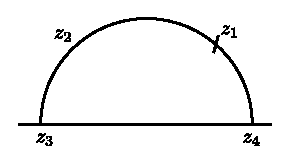
\includegraphics{fig2.eps}
\end{figure}
$$
\delta_{0}(z_{1},z_{2})=\log[D(z_{1},z_{2},z_{3},z_{4})]
$$
where $z_{3}$ and $z_{4}$ are the points in which the unique circle
through $z_{1}$ and $z_{2}$ orthogonal to the real line, intersects
the real line: $z_{1}$, $z_{2}$, $z_{3}$, $z_{4}$ being in cyclical
order and $D(z_{1},z_{2},z_{3},z_{4})$ is the cross ratio
$$
D(z_{1},z_{2},z_{3},z_{4})=\frac{z_{1}-z_{3}}{z_{1}-z_{4}}:\frac{z_{2}-z_{3}}{z_{2}-z_{4}}. 
$$
With this notation we see that \eqref{c3:eq43} can be written as 
\begin{equation*}
\delta(z_{1},z_{2})=\frac{1}{2}\log[D(z_{1},z_{2},-1,1)]\tag{45}\label{c3:eq45}
\end{equation*}
Let us now go back to the $\mathfrak{H}$ space. This consists of
points $H=H_{0}[C]$. We shall assume $|C|=1$. For if not, we
interchange the columns of $C$ which merely means taking $-S$ instead
of $S$. By \eqref{c3:eq38} it follows that 
\begin{figure}[H]
\centering
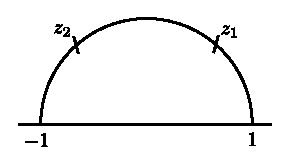
\includegraphics{fig3.eps}
\end{figure}
the $\mathfrak{H}$ space is precisely the semi-circle on $\tau_{1}$,
$\tau_{2}$ as diameter, where $\tau_{1}$, $\tau_{2}$ are the roots of
\eqref{c3:eq37}. The equation of this semi-circle is, as can be seen
\begin{equation*}
a(\xi^{2}+\eta^{2})+2b\xi+c=0\tag{46}\label{c3:eq46}
\end{equation*}
with centre on the real line at the point $-\dfrac{b}{a}$ and radius
$\sqrt{\dfrac{||S||}{a}}$. 

In\pageoriginale the previous chapter we had seen that the modular
region $F$ defined by
\begin{figure}[H]
\centering
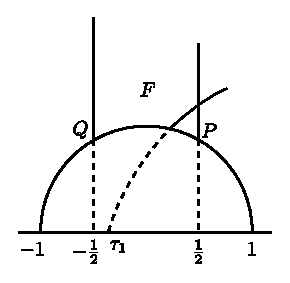
\includegraphics{fig4.eps}
\end{figure}

\begin{gather*}
z\ob{z}\geq 1\\
- \frac{1}{2}\leq \xi\leq \frac{1}{2}
\end{gather*}
is a fundamental region for the proper unimodular group. Analogous to
our definition of reduction of indefinite form in the last section, we
define a binary form $S[\ub{x}]$ {\em reduced} if its $\mathfrak{H}$
space intersects $F$ in a non-empty set. Since transformations in the
upper half plane are by means of matrices of determinant unity, this
can be called {\em proper reduction}. Since the $\mathfrak{H}$ space
is given by \eqref{c3:eq46}, the fact that $S$ is reduced means that at
least one of the vertices $P$, $Q$ lies within the circle
\eqref{c3:eq46}. Since $P$, $Q$ are the points $\dfrac{\pm 1+i\sqrt{3}}{2}$
we see that if $S$ is reduced, then
$$
a\left(\xi^{2}+\eta^{2}\right)+2b\xi+c\leq 0
$$
where $\xi=\pm \frac{1}{2}$ and $\eta=\dfrac{\sqrt{3}}{2}$. This gives
\begin{equation*}
a\pm b+c\leq 0.\tag{47}\label{c3:eq47}
\end{equation*}

We may assume $a>0$. For, if $a<0$ (we have already assumed it is not
equal to zero) there exists a properly unimodular matrix $U$ such that
the first diagonal element of $S[U]$ is positive. In this case, we
have since $a+c\leq |b|$ we get
$$
\frac{1}{4}(4a-2|b|)^{2}+3b^{2}=(2|b|-a)^{2}+3a^{2}=4d+4(a^{2}-a|b|+ac)\leq
4d
$$
where\pageoriginale $d=||S||$. This gives at once
$$
a^{2}\leq \frac{4}{3}d,\quad b^{2}\leq \frac{4}{3}d,\quad 3ac\leq d
$$
which at once shows that the number of integral properly reduced forms
of given determinant is finite.

It is to be {\em noted} that the reduction conditions above are not
the same as those of Gauss.

Let us now construct a fundamental region for the unit group in this
$\mathfrak{H}$ space. Before doing this, we shall first study the
structure of the unit group $\Gamma=\Gamma(S)$ of $S$.

Let $S[\ub{x}]=ax^{2}+bxy+cy^{2}$ be a form representing integers for
integral values of $x$ and $y$. Then
$$
S=
\begin{pmatrix}
a & b/2\\
b/2 & c
\end{pmatrix}
$$
is a semi-integral matrix. Let
$$
b^{2}-4ac=d.
$$
$d>0$ and not a square. Then $S[\ub{x}]$ is not a zero form. Also let
$(a,b,c)=1$. Since $S[\ub{x}]$ is not a zero form, neither $\ub{a}$
nor $c$ is zero. We shall consider the proper group of units $U$ of
$S$, namely the group $\Gamma_{0}=\Gamma_{0}(S)$ of unimodular
matrices $U$ such that
\begin{equation*}
S[U]=S,\quad |U|=1.\tag{48}\label{c3:eq48}
\end{equation*}
Clearly $\Gamma_{0}$ is a subgroup of $\Gamma$ of index $2$. Let
$U=\left(\begin{smallmatrix} \alpha & \beta\\ \gamma & \delta
\end{smallmatrix}\right)$ be an element of $\Gamma_{0}$. Let
$\tau_{1}$, $\tau_{2}$ be the roots of 
\begin{equation*}
a\lambda^{2}+b\lambda+c=0.\tag{49}\label{c3:eq49}
\end{equation*}\pageoriginale
Then it can be seen that the mapping $S\to S[U]$ keeps $\tau_{1}$ and
$\tau_{2}$ fixed. Thus
$$
\tau_{i}=\frac{\delta\tau_{i}-\beta}{-\gamma\tau_{i}+\alpha},i=1,2.
$$
which means that $\tau_{1}$ and $\tau_{2}$ are again roots of the
polynomial
\begin{equation*}
\gamma\lambda^{2}+(\delta-\alpha)\lambda-\beta=0\tag{50}\label{c3:eq50}
\end{equation*}
\eqref{c3:eq49} is irreducible in the rational number field since otherwise
$\tau_{1}$ and $\tau_{2}$ will both be rational and so $\sqrt{||S||}$
is rational, which is a contradiction to our assumption that
$S[\ub{x}]$ is not a zero form. Therefore \eqref{c3:eq49} and \eqref{c3:eq50}
give
\begin{equation*}
\frac{\gamma}{a}=\frac{\delta-\alpha}{b}=\frac{-\beta}{c}=q\tag{51}\label{c3:eq51}
\end{equation*}
where $q$ is an integer. If $U\neq \pm E$ then $\gamma\neq 0$,
$\beta\neq 0$. Let us put $\delta+\alpha=p$. Then
\begin{equation*}
\delta=\frac{p+bq}{2},\quad \alpha=\frac{p-bq}{2}\tag{52}\label{c3:eq52}
\end{equation*}
Since $\alpha\delta-\beta\gamma=1$, we get the relation
$\dfrac{p^{2}-q^{2}b^{2}}{4}+q^{2}ac=1$ or
\begin{equation*}
\boxed{p^{2}-dq^{2}=4}\tag{53}\label{c3:eq53}
\end{equation*}
which is the well-known Pell's equation. Thus every unit of $S$ in
$\Gamma_{0}$ gives rise to a solution of Pell's equation. Conversely
every solution of \eqref{c3:eq53} gives rise to a unit $U$ of $S$, as can
be seen\pageoriginale from \eqref{c3:eq51} and \eqref{c3:eq52}. This unit is
$$
U=
\begin{pmatrix}
\dfrac{p-bq}{2} & -cq\\[10pt]
aq & \dfrac{p+bq}{2}
\end{pmatrix}
$$

Consider the representation $H\to H[U]$, $U\in\Gamma_{0}$ in the
$\mathfrak{H}$ space. Let the representative point of $H_{0}$ be
$z_{0}$ on the semi-circle which defines the $\mathfrak{H}$
space. Denote by $w_{0}$ the point $H_{0}[U]$. Let $z$ be any variable
point on this semi-circle and $w$ the image by the transformation
$H\to H[U]$. If $U=\left(\begin{smallmatrix}\alpha & \beta\\ \gamma &
  \beta
\end{smallmatrix}\right)$ then
$$
w_{0}=\frac{\delta z_{0}-\beta}{-\gamma z_{0}+\alpha},\quad
W=\frac{\delta z-\beta}{-\gamma z+\alpha}.
$$
Because of the fact that $U$ fixes both $\tau_{1}$ and $\tau_{2}$ and
cross-ratio is unaltered by linear transformation, we see that
$$
\frac{z-\tau_{1}}{z-\tau_{2}}:\frac{z_{0}-\tau_{1}}{z_{0}-\tau_{2}}=\frac{w-\tau_{1}}{w-\tau_{2}}:\frac{w_{0}-\tau_{1}}{w_{0}-\tau_{2}} 
$$
or that
\begin{equation*}
\frac{w-\tau_{2}}{w-\tau_{1}}=\mu
\frac{z-\tau_{2}}{z-\tau_{1}}\tag{54}\label{c3:eq54} 
\end{equation*}
where $\mu=D(w_{0},z_{0},\tau_{1},\tau_{2})$. But equation \eqref{c3:eq54}
shows that $\mu=D(w,z,\break\tau_{1},\tau_{2})$, which means that $\mu$ is a
constant independent of the point $z$. This shows that in the
non-Euclidean geometry of ours, the mapping $H\to H[U]$ corresponds to
a translation. Also (See \cite{c3:key11}) the quantity $\mu$ has the
property that if\pageoriginale $\lambda_{1}$ and $\lambda_{2}$ are the
eigen values of the matrix of the transformation
\begin{equation*}
w=\frac{\delta z-\beta}{-\gamma z+\alpha}\tag{55}\label{c3:eq55}
\end{equation*}
then, by proper ordering of $\lambda_{1}$ and $\lambda_{2}$ we have
$$
\mu=\frac{\lambda_{1}}{\lambda_{2}}
$$
and therefore the non-Euclidean distance $\delta_{0}(z,w)$ is given by 
$$
\delta_{0}(z,w)=\log\frac{\lambda_{1}}{\lambda_{2}}
$$
where $\lambda_{1}\geq\lambda_{2}$. Now $\lambda_{1}$ and
$\lambda_{2}$ are characteristic roots of the mapping \eqref{c3:eq55} and
hence they satisfy
$$
\lambda^{2}-(\alpha+\delta)\lambda+1=0
$$
which shows that
$$
\lambda_{1},\lambda_{2}=\frac{\alpha + \delta}{2}\pm
\sqrt{\left(\dfrac{\alpha+\delta}{2}\right)^2 -1.}
$$
Substituting from \eqref{c3:eq52}, $\alpha+\delta=p$, we get
\begin{equation*}
\lambda_{1},\lambda_{2}=\frac{p\pm q\sqrt{d}}{2}\tag{56}\label{c3:eq56}
\end{equation*}
where $p$ and $q$ are the unique solutions of Pell's equation
corresponding to the unit $U$.

Let $R$ be the field of rational numbers and $R(\sqrt{d})$ the real
quadratic field. The element $\varepsilon$ of $R(\sqrt{d})$ defined by
$$
\varepsilon=\frac{p+q\sqrt{d}}{2}
$$
where\pageoriginale $p$ and $q$ are a solution of Pell's equation, is
a unit of norm 1. This is seen from the fact that $\varepsilon$ is a root
of
$$
\lambda^{2}-p\lambda+1=0.
$$
(If $d$ is square-free the converse is also true).

In \eqref{c3:eq56}, the quantities $\lambda_{1}$, $\lambda_{2}$ are
$\varepsilon$ and $\varepsilon^{-1}$ in some order. If $U$ is changed to
$U^{-1}$ or to $-U$, then $\varepsilon$ gets changed to $\varepsilon^{-1}$
or $-\varepsilon$ respectively. We therefore choose among the four
quantities $\varepsilon$, $-\varepsilon$, $\varepsilon^{-1}$, $-\varepsilon^{-1}$,
one (and there is only one in general), call it $\varepsilon^{\ast}$
which is such that 
$$
\varepsilon^{\ast}\geq 1
$$
and put 
$$
\delta_{0}(z,w)=\log \varepsilon^{\ast 2}.
$$
(Note that $\lambda_{1}/\lambda_{2}=\varepsilon^{\ast 2}$ with
$\lambda_{1}\geq \lambda_{2}$). This will then mean that the
translation in the $\mathfrak{H}$ space is by the amount 
$$
\delta(z,w)=\log \varepsilon^{\ast}.
$$

Since the representation of $\Gamma_{0}$ in $\mathfrak{H}$ is
discontinuous it follows that the translations form a discrete
subgroup in the group of non-Euclidean motions on
$\mathfrak{H}$. There is thus a $U_{0}$ and a corresponding
$\varepsilon^{\ast}_{0}$ such that $\log \varepsilon^{\ast}_{0}$ is the
smallest. Hence any $U$ will be of the form 
$$
U=\pm U^{n}_{0}\quad (n=0,\pm 1,\ldots)
$$
Similarly any $\varepsilon$ which arises from a $U$ in $\Gamma_{0}$ is of
the form
$$
\varepsilon=\pm \varepsilon^{\ast n}_{0}\quad (n=0,\pm 1,\ldots)
$$

If\pageoriginale instead of $S$ being semi-integral, it was rational
symmetric we could, by multiplying it by an integer, make it integral
satisfying the condition $(a,b,c)=1$. But this multiplication does not
affect the unit group. Hence the

\begin{thm}\label{chap3:thm4}
The group of proper units of an indefinite, binary, non-zero, rational
quadratic form is an infinite cyclic group whose elements stand in
$a(1,1)$ correspondence with the solutions of Pell's equation.
\end{thm}

Let $S=\left(\begin{smallmatrix} a & b\\ b &
  c\end{smallmatrix}\right)$ be a rational symmetric, non-singular
  indefinite matrix and let $S[\ub{x}]$ be not a zero form. Let the 
\begin{figure}[H]
\centering
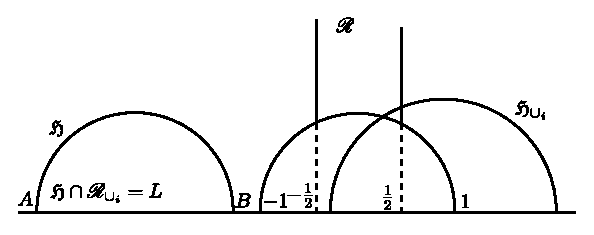
\includegraphics{fig5.eps}
\end{figure}
semi-circle $ALB$ denote the $\mathfrak{H}$ space of the matrix $S$ so
that $A$ and $B$ are points on the real axis with coordinates
$\tau_{2}$ and $\tau_{1}$, $\tau_{2}\neq \tau_{1}$. Furthermore since
$S[\ub{x}]$ is not a zero form, the quantities $\tau_{1}$ and
$\tau_{2}$ are irrational. Let $\mathscr{R}$ denote the fundamental
region of the proper unimodular group in the upper half $z$-plane. Let
$U_{1},\ldots,U_{g}$ be the finitely many reducing properly
unimodular\pageoriginale matrices. If $\mathfrak{H}_{U}$ for
$U=U_{1},\ldots,U_{g}$ denotes the image of $\mathfrak{H}$ under the
transform $H\to H[U]$ (this means for the points $z$ on $\mathfrak{H}$
the transformation $z\to \dfrac{\varepsilon_{z}-\beta}{-\gamma
  z+\alpha}$, $U=\left(\begin{smallmatrix} \alpha & \beta\\ \gamma &
  \delta
\end{smallmatrix}\right)$), then
$$
G=\sum^{g}_{i=1}(\mathfrak{H}_{U_{i}}\cap \mathscr{R})_{U_{i}^{-1}}
$$
is a point set on $\mathfrak{H}$ and is a fundamental region for
$\Gamma_{0}$ in $\mathfrak{H}$. It is important to notice that
$\mathfrak{H}_{U_{i}}$ does not lie completely on the boundary of
$\mathscr{R}$. For then $\mathfrak{H}_{U_{i}}$ would have to be the
unit circle or one of the lines $\xi=\pm 1/2$. In the first case this
would mean that
$$
\frac{\delta z-\beta}{-\gamma z+\alpha}=\pm 1
$$
where $z=\tau_{1}$ or $\tau_{2}$. This is the same as saying
$\tau_{1}$ and $\tau_{2}$ are rational, which they are not. Then same
happens if the second case is true.

This shows that none of the arcs $(\mathfrak{H}_{U_{i}}\cap
\mathscr{R})_{U_{i}}$ has an end point at $\tau_{1}$ or
$\tau_{2}$. Hence $G$ is compact. Its volume therefore in the measure
induced by the invariant metric is finite.


\begin{thebibliography}{99}
\bibitem{c3:key1}  E.\@ Cartan : Sur une classe remarquable $d'$
  espaces de Riemann, 
{\em Bull.\@ Math.\@ Soc.\@ France}, Tome 55 (1927) P.\@ 114 -
134.

\bibitem{c3:key2} Fricke-Klein :\pageoriginale  {\em Vorlesungen
  \"uber die theorie der 
  Modul}-funktionen, Bd.1, Leipsig (1890), P.243-269.

\bibitem{c3:key3} C. F. Gauss :  {\em Disquisitiones Arithmeticae.}

\bibitem{c3:key4} C.\@ Hermite : {\em Oeuvres}, Tome 1, Paris (1905),
P.164-293.

\bibitem{c3:key5} L.\@ Pontrjagin :  {\em Topological groups}, Princeton
(1940).

\bibitem{c3:key6} C.\@ L.\@ Siegel :  Discontinuous groups, {\em Annals
  of Math}., 44 (1943), P.\@ 674-689.

\bibitem{c3:key7} C.\@ L.\@ Siegel :  Some remarks on discontinuous groups, {\em
  Annals of Math}., 46(1945), P.708-718.

\bibitem{c3:key8} C.\@ L.\@ Siegel :  Einheiten quadratischer Formen, {\em Abh.\@
  aus.\@ dem.\@ Math.\@ Semi.\@ Hansischen Univ}., 13(1940),
P.209-239.

\bibitem{c3:key9} C.\@ L.\@ Siegel : Indefinite quadratische Formen und
Funktionentheorie I, {\em Math.\@ Annalen}, 124 (1951),
P.17-54.

\bibitem{c3:key10} C.\@ L.\@ Siegel :  The average measure of quadratic forms with
given determinant and signature, {\em Annals of Math}., 45(1944),
P.667-685.

\bibitem{c3:key11} C.\@ L.\@ Siegel :  {\em Ausgew\"ahlte Fragen der
  Funktionentheorie II} G\"ottingen, 1953.

\bibitem{c3:key12} A.\@ Weil : {\em L'int\'egration dans les groupes topologiques
  et ses applications}, Paris (1940).  
\end{thebibliography}
